%TODO: Die Schätzungen gehen nur von Veränderungen der verwendeten Menge bzgl.
%Transistoren aus. Wenn diese Menge nur ein Bruchteil ausmacht, dann hat auch
%die Verwendung einer Alternative kaum einen Einfluss. Das müssen wir noch
%irgendwie berücksichtigen.

\section{Wirtschaftlich}\label{sec:conflict}

Dieser Abschnitt beschreibt die wirtschaftliche Nachhaltigkeit von Tantal für alle abgehandelten Szenarien. Die Nachhaltigkeitsanalyse beschäftigt sich dabei mit dem globalen Effekt des Tantalabbaus.

\subsection{Indikatoren}

\paragraph{Preis}
Mittels Indikator ``Preis'' untersucht man, wie sich der Preis pro Kilo Tantal
in amerikanischen Dollars (USD) verändert. Eine Senkung wird als positiv bewertet, da die ICT-Branche von günstigeren Rohstoffpreisen profitiert. 

\paragraph{Arbeitsplätze}
Der Indikator ``Arbeitsplätze'' misst, wie die Produktion von Tantal die Anzahl
Arbeitsplätze beeinflusst. Die Qualität der Arbeitsplätze ist bei diesem Indikator kein Kriterium. Eine Erhöhung der Anzahl Arbeitsplätze wird als positiv bewertet.

\paragraph{Innovation}
Dieser Indikator misst, ob durch die Produktion von Tantal neue Technologien
entstehen und ob diese nachhaltig die Marktentwicklung beeinflussen können. Steigt das Innovationspotential, steigt auch die Bewertung des Indikators.

\subsection{Bewertung}

\paragraph{2013}
Der \textbf{Preis} von Tantal pro Kilogramm betrug im Jahr 2006 USD 65.-, 2010 USD 121.- und 2013 USD 237.- ~\cite{tantal_price2}. 237.- USD führt auf der Nachhaltigkeitsskala zu einer neutralen 5.

\begin{figure}[h]
\centering
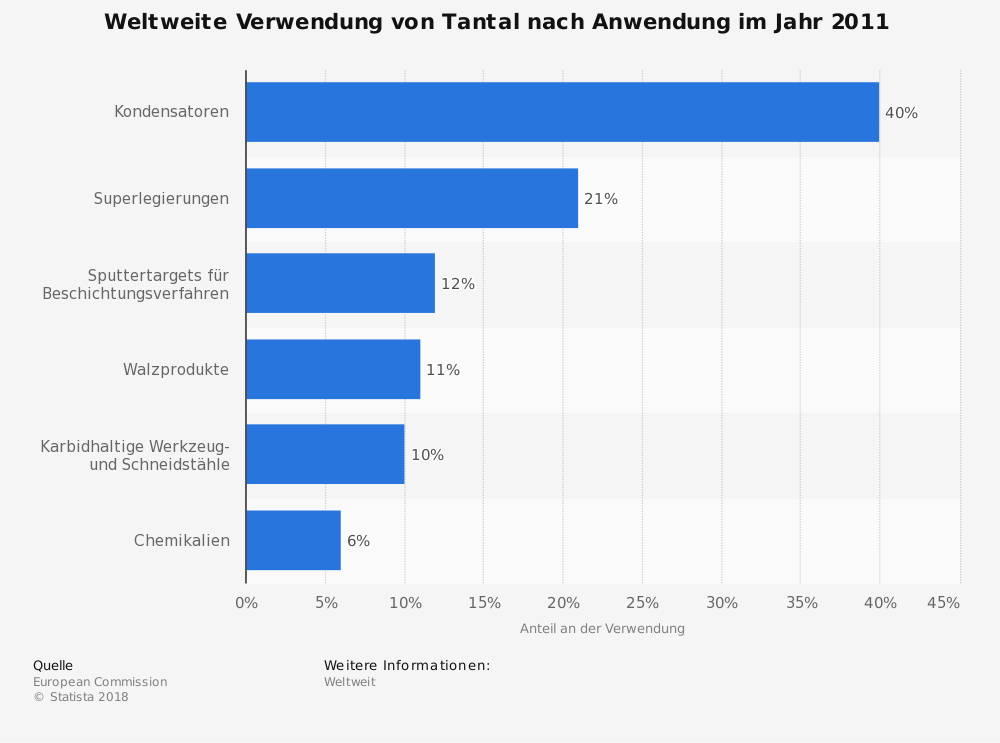
\includegraphics[width=0.8\textwidth]{tantal_usage_2011}
\caption{BGR. n.d. Weltweite Verwendung von Tantal nach Anwendung im Jahr 2011 ~\cite{tantal_usage}}
\label{}
\end{figure}

Bergwerke haben 2013 weltweit 1300 Tonnen Tantal gefördert ~\cite{tantal_price2}. 2011 wurden 40\% des geförderteten Tantals für Kondensatoren verwendet.~\cite{tantal_usage} Bei gleichbleibender Verwendungsrate entspricht dies einer Fördermenge von 520 Tonnen im Jahr 2013. 2010 wurden weltweit 779 Tonnen gefördert ~\cite{tantal_price2}. Dies entspricht einer Förderungszunahme von 521 Tonnen. Unter der Annahme, dass die Anzahl Arbeitsplätze in der Metall-Förderbranche direkt mit der absoluten, weltweiten Fördermenge korreliert, hat sich diese Anzahl positiv entwickelt. 
Da die Nachfrage und somit der Abbau von Tantal stetig steigt~\cite{tantal_price2}, werden auch konstant neue Arbeitsplätze geschaffen. Dieser Trend ist positiv und wird mit einer 6 bewertet.

Tantal ist ein essentieller Bestandteil von Kondensatoren, die für Mikroprozessoren benötigt werden. Mikroprozessoren finden Verwendung in Computern und Maschinensteuerungen. Die Leistungsfähigkeit dieser Mikroprozessoren steigt jährlich und sorgt somit für eine anhaltende Innovation. Der Indikator \textbf{Innovation} wird deshalb mit einer 7 bewertet.

\paragraph{2035 bei anhaltendem Trend}
Bei steigender Tantalnachfrage wird der \textbf{Preis} ebenfalls weiterhin steigen. Von 2006 bis 2013 ist dieser um 364.62\% gestiegen ~\cite{tantal_price2}. Rechnet man diese Entwicklung hoch (jährlicher Preisanstieg um 24.5 USD), beträgt der Preis 2035 etwa 775 USD. Dieser starke Preisanstieg wirkt sich negativ auf die Wirtschaft aus und wird mit einer 1 bewertet.

Die Nachfrage beeinflusst auch die Anzahl \textbf{Arbeitsplätze}. Bis 2035 ist damit zu rechnen, dass sich die Nachfrage von Tantal verdoppelt. Damit keine Engpässe entstehen, braucht es weitere Minen und mehr Arbeitsplätze. Bereits im Jahr 2018 starten neue Minen in Australien den Abbau von Tantal.~\cite{new_mine_aus} Diese positive Entwicklung führt zu einer 8 auf der Nachhaltigkeitsskala.

Da technologisch keine Veränderung in diesem Szenario ersichtlich ist, wird die Innovation mit einer 6 leicht schlechter als 2013 bewertet.

\paragraph{2035 mit Kondensatorenalternative}
Obwohl eine Alternative für die Kondensatoren eine Entlastung des Tantalbedarfs in der ICT-Branche bedeutet, benötigen weiterhin andere Industrien Tantal. Wenn der Anteil von 40\% der Tantalproduktion, welche für Kondensatoren verwendet werden, wegfällt, müssen dennoch 305 Tonnen mehr als im Jahr 2013 gefördert werden.~\cite{tantal_price2} Der \textbf{Preis} wird somit leicht steigen und erhält eine 4 auf der Nachhaltigkeitsskala.

Wegen der wegfallenden Tantalnachfrage für Kondensatoren steigt die Gesamtnachfrage weniger steil an wie in der Prognose mit anhaltendem Trend. Die Gesamtnachfrage wird jedoch steigen und mehr \textbf{Arbeitsplätze} entstehen. Der Nachhaltigkeitsindex erhält eine 7.

Eine Technologie, welche zur Herstellung von Kondensatoren kein Tantal mehr benötigt, ist innovativ und wird eine Reihe von neuen Innovationen auslösen. Diese Innovationen werden vergleichbar sein mit der anhaltenden Leistungssteigerung der Mikroprozessoren. Da Innovationen für eine gesunde Wirtschaft sehr wichtig sind, wird der Indikator mit einer 8 bewertet.

\begin{table}[h]
  \centering
  \begin{tabular}{l|ccc}            & \textbf{2013} & \textbf{2035} & \textbf{2035 mit Annahme}
    \\ \hline Preis                 & 5             & 1             & 4
    \\ Arbeitsplätze                & 6             & 8             & 7
    \\ Innovation                   & 7             & 6             & 8
    \\ \hline \textbf{Endbewertung} & 6             & 5             & 6\(\frac{1}{3}\)
  \end{tabular}
  \caption{Resultat wirtschaftliche Analyse}
\end{table}
